\documentclass[a4paper,12pt]{article} % тип документа

% Поля страниц
\usepackage[left=2.5cm,right=2.5cm,
    top=2cm,bottom=2cm,bindingoffset=0cm]{geometry}
    
%Пакет дял таблиц   
\usepackage{multirow} 
    
%Отступ после заголовка    
\usepackage{indentfirst}


% Рисунки
\usepackage{floatrow,graphicx,calc}
\usepackage{wrapfig}

%%% Работа с картинками
\usepackage{graphicx}  % Для вставки рисунков
\graphicspath{{images/}}  % папки с картинками
\setlength\fboxsep{3pt} % Отступ рамки \fbox{} от рисунка
\setlength\fboxrule{1pt} % Толщина линий рамки \fbox{}
\usepackage{wrapfig} % Обтекание рисунков и таблиц текстом

% Создаём новый разделитель
\DeclareFloatSeparators{mysep}{\hspace{1cm}}

% Ссылки?
\usepackage{hyperref}
\usepackage[rgb]{xcolor}
\hypersetup{				% Гиперссылки
    colorlinks=true,       	% false: ссылки в рамках
	urlcolor=blue          % на URL
}


%  Русский язык
\usepackage[T2A]{fontenc}			% кодировка
\usepackage[utf8]{inputenc}			% кодировка исходного текста
\usepackage[english,russian]{babel}	% локализация и переносы

% Математика
\usepackage{amsmath,amsfonts,amssymb,amsthm,mathtools}

%%% Дополнительная работа с математикой
\usepackage{amsmath,amsfonts,amssymb,amsthm,mathtools} % AMS
\usepackage{icomma} % "Умная" запятая: $0,2$ --- число, $0, 2$ --- перечисление

% Что-то 
\usepackage{wasysym}


\begin{document}
\begin{center}
	\footnotesize{ФЕДЕРАЛЬНОЕ ГОСУДАРСТВЕННОЕ АВТОНОМНОЕ ОБРАЗОВАТЕЛЬНОЕ 			УЧРЕЖДЕНИЕ ВЫСШЕГО ОБРАЗОВАНИЯ}\\
	\footnotesize{МОСКОВСКИЙ ФИЗИКО-ТЕХНИЧЕСКИЙ ИНСТИТУТ\\(НАЦИОНАЛЬНЫЙ 			ИССЛЕДОВАТЕЛЬСКИЙ УНИВЕРСИТЕТ)}\\
	\footnotesize{ФИЗТЕХ-ШКОЛА ФИЗИКИ И ИССЛЕДОВАНИЙ им. ЛАНДАУ\\}
	\hfill \break
	\hfill \break
	\hfill \break
	\hfill \break
\end{center}

\begin{center}   
    \hfill \break
	\hfill \break
	\hfill \break
	\hfill \break    \hfill \break
	\hfill \break
	\hfill \break
	\hfill \break
    \hfill \break
    \hfill \break
	\hfill \break
	\large{Лабораторная работа № 2.4.1\\\textbf{Определение теплоты испарения жидкости}}\\
	\begin{flushright}
		Плотникова Анастасия Александровна\\
		Группа Б02-406
	\end{flushright}
	\hfill \break
	\hfill \break
	\hfill \break
\end{center}
\hfill \break
\hfill \break
\hfill \break
\hfill \break
\hfill \break
\hfill \break
\hfill \break
\hfill \break
\hfill \break
\hfill \break
\hfill \break
\hfill \break
\hfill \break
\begin{center}
	Долгопрудный, 2025 г.
\end{center}
\thispagestyle{empty}
\newpage
	\textbf{Цель работы:}\\ 1) измерение давления насыщенного пара жидкости при разной температуре;\\ 2) вычисление по полученным данным теплоты испарения с помощью уравения Клапейрона-Клаузиуса.
	\hfill \break
	
	\textbf{В работе используются:}\\ термостат,\\ герметический сосуд, заполненный водой,\\ отсчетный микроскоп.
	
\section{Теоретическая справка}

\textit{Испарение} — переход вещества из жидкого в газообразное состояние на свободной поверхности жидкости. 

Для выхода из жидкости молекуля должны совершить работу против сил молекулярного сцепления, внешнего давления, для чего должны обладать достаточной кинетической энергией. Переход части быстрых молекул в пар сопровождается потерями энергии, следовательно, и охлаждением жидкости.

\textit{Молярная теплота испарения (парообразования)} — количество теплоты, необходимое для изотермического испарения одного моля жидкости при внешнем давлении, равном упругости ее насыщенных паров.
    
В настоящей работе для определения теплоты испарения применен косвенный метод, основанный на формуле Клапейрона-Клаузиуса:
\begin{equation}
    \label{Klap}
    \frac{dP}{dT} = \frac{L}{T(V_2 - V_1)}
\end{equation}

\noindent $P$ -- давление насыщенного пара жидкости при температуре $T$,\\ $T$ -- абсолютная температура жидкости и пара,\\ $L$ — теплота испарения жидкости,\\ $V_2$ -- объем пара,\\ $V_1$ -- объем жидкости.

\begin{table}[h]
  \centering
  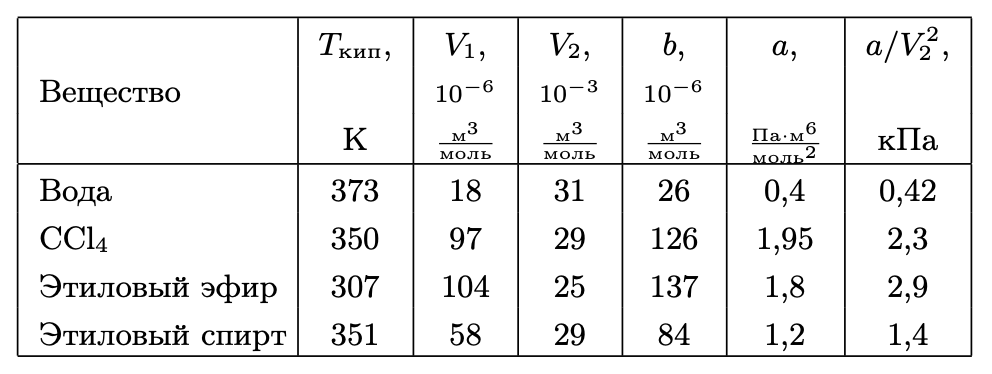
\includegraphics[scale = 0.55]{table_data.png}
  \caption{Табличные данные}
  \label{fig:table_data}
\end{table}

Найдя из опыта $dP/dT$, $T$, $V_2$ и $V_1$, можно определить $L$ путем расчета. Величины $L$, $V_2$ и $V_1$ в формуле (\ref{Klap}) должны относиться к одному и тому же количеству вещества; мы будем относить их к одному молю.

Измерения проводятся при давлениях ниже атмосферного.

Из табличных данных видно, что $V_1$ не превосходит $0.5\%$ от $V_2$. 

\medskip

Обратимся теперь к $V_2$, которое в дальнейшем будем обозначать $V$. Объем $V$ связан с давелнием и темературой уравнением Ван-дер-Ваальса:

\begin{equation}
    \label{Van-der}
    \left( P + \frac{a}{V^2}\right)(V - b) = RT
\end{equation}

Из рассмотрения таблицы (\ref{fig:table_data}) следует, что $b$ одного порядка с $V_1$. В уравнении Ван-дер-Ваальса величиной $b$ следует пренебречь. Пренебрежение членом $a/V^2$ по сравнению с $P$ вносит ошибку менее 3\%. При давлении ниже атмосферного ошибки становятся еще меньше. Таким образом, при давлениях ниже атмосферного уравнение Ван-дер-Ваальса для насыщенного пара мало отличается от уравнения Клапейрона. Положим поэтому

\begin{equation}
    \label{ideal}
    P = \frac{RT}{V}
\end{equation}

Подставляя (\ref{ideal}) в (\ref{Klap}) и разрешая уравение относительно $L$, получаем:

\begin{equation}
    \label{L}
    L = \frac{RT^2}{P}\frac{dP}{dT} = -R\frac{d(\mbox{ln }P)}{d(1/T)}
\end{equation}

Эта формула является окончательной.

\section{Экспериментальная установка}

Схема установки изображена на рисунке (\ref{fig:drawing1}). 

\begin{figure}[h]
  \centering
  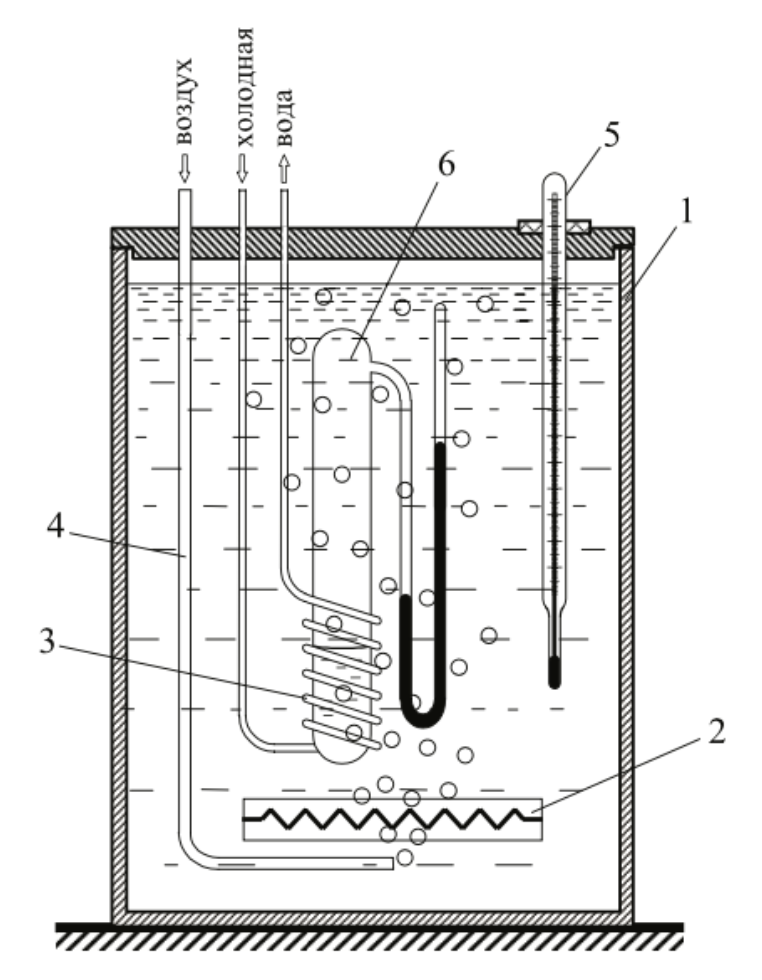
\includegraphics[scale = 0.5]{drawing1.png}
  \caption{Схема установки для определения теплоты испарения}
  \label{fig:drawing1}
\end{figure}

\begin{enumerate}
  \item Наполненный водой резервуар (термостат);
  \item Спираль, подогреваемая электрическим током. Нагревает термостат.
  \item Змеевик, через который пропускается водопроводная вода для охлаждения воды в термостате.
  \item Трубка. Через нее поступает воздух, перемешивающий воду в термостате.
  \item Термометр.
  \item Запаянный прибор с исследуемой жидкостью. Над ней находится насыщенный пар (перед заполнением прибора воздух из него был откачан).
\end{enumerate}

Давление насыщенного пара определяется по ртутному манометру, соединенному с исследуемым объемом. 

Отсчет показаний манометра производится при помощи микроскопа. 

\bigskip
В эксперименте $T$ и $P$ определяются термометром и манометром, соответственно. Производные $\frac{dP}{dT}$ и $\frac{d(\mbox{ln }P)}{d(\frac1T)}$ можно найти из углового коэффициента касательной к графику $P(T)$ или как коэффициент наклона прямой на графике с осями ln $P$ и $\frac1T$.

\section{Ход эксперимента}

\begin{enumerate}
  \item Измерили разность уровней в ртутном U-образном манометре с помощью микроскопа. Измерим температуру термометром. Полученные значения занесем в таблицу (\ref{tab:init}).
  \item Включили термостат. Подогревали воду в калориметре, пропуская ток через нагреватель. Следили за тем, чтобы воздух всё время перемешивал воду. \\ Через каждые 1-3 градуса измеряли давление и температуру. Результаты занесли в таблицу (\ref{tab:heating}). \\ Повышали температуру в течение ??, чтобы успеть произвести измерения при остывании прибора.
  \item Провели те же измерения при охлаждении жидкости. Установили такой поток воды, чтобы охлаждение шло примерно тем же темпом, что и нагревание. Результаты измерений в таблице (\ref{tab:cooling}).
  \item Построили графики в координатах $T$, $P$ и в координатах $1/T$, $ln P$. % На графики нанесли точки, полученные при нагревании и охлаждении жидкости (разными цветами).
  \item Вычислили $L$, пользуясь формулой (\ref{L}) и данными, полученными сначала из одного, а потом из другого графика. \\ Сравнили результаты, оценили ошибку измерений.
\end{enumerate}
\section{Результаты измерений}

$\rho_{Hg} = 13600$ кг/м$^3$

$P = 2\rho g\Delta h$, где $\Delta h = h_2 - h_1$ — разность высот столбов ртути

\medskip

Графики зависимости давления от температуры представлены на Рис.\ref{fig:graph1} и Рис.\ref{fig:graph2}.

Из графика \ref{fig:graph1} хорошо видно, что зависимость не линейная. 

\begin{table}[h]
    \caption{Начальные измерения}
    \centering
        \begin{tabular}{|c|c|c|c|c|}
     \hline $T_{0}$, $^\circ$C & $P_{0}$, Па & $h_1$, мм & $h_2$, мм & $\delta h$, мм \\
    \hline  &  &  &  &  \\
    \hline
\end{tabular}
    \label{tab:init}
\end{table}
\begin{table}[h]
    \caption{Измерения при нагреве}
    \begin{tabular}{|c|c|c|}
        \hline $T$, $^\circ C$  &  $\Delta h$, мм & $P$, Па \\
        \hline  &  &  \\
        \hline  &  &  \\
        \hline  &  &  \\
        \hline  &  &  \\
        \hline  &  &  \\
        \hline  &  &  \\
        \hline  &  &  \\
        \hline  &  &  \\
        \hline  &  &  \\
        \hline  &  &  \\
        \hline
    \end{tabular}
    \label{tab:heating}
\end{table}
\begin{table}[h]
    \caption{Измерения при охлаждении}
    \begin{tabular}{|c|c|c|}
        \hline $T$, $^\circ C$  &  $\Delta h$, мм & $P$, Па \\
        \hline  &  &  \\
        \hline  &  &  \\
        \hline  &  &  \\
        \hline  &  &  \\
        \hline  &  &  \\
        \hline  &  &  \\
        \hline  &  &  \\
        \hline  &  &  \\
        \hline  &  &  \\
        \hline  &  &  \\
        \hline 
    \end{tabular}
    \label{tab:cooling}
\end{table}

\section{Вывод}
\end{document}
